% !TeX program = xelatex
\documentclass[12pt,a4paper]{article}
\usepackage{fontspec}
\setmainfont{Times New Roman}
\setsansfont{Arial}
\setmonofont{Courier New}
\usepackage[english,russian]{babel}
\usepackage{amsmath,amssymb}
\usepackage[margin=22mm]{geometry}
\usepackage{graphicx,float}
\usepackage[unicode,hidelinks]{hyperref}
\setlength{\emergencystretch}{3em}
\interfootnotelinepenalty=10000
\newcommand{\topic}[1]{\par\medskip\noindent\textbf{#1}\par\nobreak\smallskip}
\renewcommand{\thefootnote}{\arabic{footnote})}
\DeclareMathOperator{\grad}{grad}
\title{Вопрос 5. Плоская установившаяся фильтрация. Методы ТФКП}
\author{Н. Е. Леонтьев\\\large Основы теории фильтрации}
\date{Учебное пособие. 2-е издание. Москва: МАКС Пресс, 2017\\Глава II, § 8. Печатные страницы 43--54}
\begin{document}
\maketitle
\noindent\textit{Полный перенос § 8, до заголовка § 9 на странице 54. Страницы PDF совпадают с печатными. Размещение материала перевёрстано. Отдельным приложением включён фрагмент рукописного конспекта о трубе-источнике.}
% Источник: Leontiev-2017.pdf; печатная страница: 43; страница файла: 43
\section*{Глава II. Фильтрация несжимаемой жидкости в недеформируемой пористой среде}
\subsection*{§ 8. Применение методов теории функций комплексного переменного для решения плоских фильтрационных задач}
\label{q5:sec-8}
Во многих практически важных случаях фильтрационные течения можно приближенно рассматривать как \textit{плоскопараллельные}, что дает возможность перейти от трехмерной задачи к двумерной и позволяет, как и в случае плоских течений идеальной несжимаемой жидкости, эффективно использовать аппарат теории функций комплексного переменного.

Типичный пример таких явлений --- движение жидкости в поперечных сечениях протяженных объектов: фильтрация под плотинами гидроэлектростанций и другими гидротехническими сооружениями (рис. 1), просачивание жидкости через земляные плотины (рис. 9~\textit{а}), отток жидкости через дно рек и каналов и т.п. Другим важным примером явлений, в которых применима модель плоскопараллельного течения, служит фильтрация в горизонтальных пластах в недрах земли. Образно выражаясь, в первом случае фильтрационное течение рассматривается при взгляде «сбоку», а во втором случае --- при взгляде «сверху».

% Источник: Leontiev-2017.pdf; печатная страница: 44; страница файла: 44
\topic{Плоскопараллельная фильтрация в вертикальной плоскости}
Рассмотрим плоское фильтрационное течение тяжелой несжимаемой жидкости в вертикальном поперечном сечении \textit{однородной} пористой среды. Направив оси $x$ и $y$ соответственно горизонтально и вертикально, можно записать систему уравнений в виде
\[
\triangle\varphi(x,y)=0,\qquad \boldsymbol{u}=(u(x,y);v(x,y))=\grad\varphi,
\]
где введен \textit{потенциал скорости фильтрации}
\begin{equation}
\varphi(x,y)\equiv-CH=-C\left(\frac{p(x,y)}{\rho g}+y\right),\qquad C=\mathrm{const}.
\tag{8.1}\label{q5:eq-8-1}
\end{equation}
Задача свелась к нахождению решения двумерного уравнения Лапласа, поэтому удобно рассматривать плоскость $Oxy$ как плоскость комплексного переменного $z=x+iy$, а потенциал $\varphi$ --- как действительную часть \textit{комплексного потенциала течения} --- аналитической функции $w(z)=\varphi(x,y)+i\psi(x,y)$, где $\psi(x,y)$ --- \textit{функция тока}, удовлетворяющая уравнениям Коши--Римана (Д’Аламбера--Эйлера) [9]
\[
\frac{\partial\varphi}{\partial x}=\frac{\partial\psi}{\partial y},\qquad
\frac{\partial\varphi}{\partial y}=-\frac{\partial\psi}{\partial x}.
\]
Задание комплексного потенциала полностью определяет фильтрационное течение, т.к. зная $w(z)$ можно найти распределение давления из \eqref{q5:eq-8-1} и распределение скорости фильтрации с помощью формулы $\frac{dw}{dz}=v-iu$, поэтому решение конкретной краевой задачи сводится к нахождению функции $w(z)$, удовлетворяющей заданным краевым условиям на границах области течения (известных или неизвестных).
% Сохранена запись оригинала dw/dz=v-iu; далее в книге используется u-iv.

Основная идея применения методов комплексного анализа при нахождении функции $w(z)$ состоит в том, что по известным условиям на границе области (в физической плоскости $z$) можно сразу сказать, каким условиям будет удовлетворять образ границы при отображениях $w(z)$, $\frac{dw(z)}{dz}$ или каких-то других (например, в зависимости от типа границы, указать значение мнимой части $w(z)$ или найти связь действительной и мнимой частей $\frac{dw(z)}{dz}$). Основываясь на этой информации можно построить конформное отображение области течения на какой-либо из ее образов или (если
% Источник: Leontiev-2017.pdf; печатная страница: 45; страница файла: 45
область течения заранее неизвестна) найти отображение одного образа на другой. Это конформное отображение дает либо сразу искомую функцию (если область в плоскости $z$ отображается на плоскость $w$), либо обыкновенное дифференциальное уравнение, из которого находится $w(z)$.

Покажем, к каким условиям на $w(z)$ и $\frac{dw(z)}{dz}$ приводят физические требования на некоторых типах границ, обсуждавшихся в § 6.

\topic{Непроницаемая граница}
\setcounter{footnote}{0}
На непроницаемой границе, так же как и в гидродинамике идеальной несжимаемой жидкости, постоянна мнимая часть комплексного потенциала: $\operatorname{Im}w=\psi=\mathrm{const}$. Значение константы на конкретной поверхности может либо определяться из условия задачи\footnote{Напомним, что разность значений функции тока в двух точках (внутри односвязной области) равна расходу жидкости через любую кривую, соединяющую точки.}, либо находиться из решения. В силу того, что функция тока определена с точностью до константы (физический смысл имеют ее пространственные производные), значение $\psi$ в одной точке можно задать произвольно.

Если участок границы является \textit{прямолинейным}, то вектор скорости фильтрации направлен вдоль границы. Поэтому в плоскости годографа\footnote{Годограф (греч. $o\delta o\varsigma$ --- «путь», «движение», $\gamma\rho\alpha\varphi\omega$ --- «пишу») --- геометрическое место концов векторов скорости, откладываемых от начала координат. Плоскость годографа $(u;v)$ получается из плоскости $\frac{dw}{dz}=(u;-v)$ отражением относительно горизонтальной оси.} этой границе соответствует прямая, проходящая через начало координат и параллельная\footnote{Если считать совпадающими ориентации осей координатных систем $(x;y)$ и $(u;v)$.} границе.

\topic{Граница с водоемом}
На границах этого типа значение напора $H$, а следовательно, и потенциала $\varphi$, является постоянной величиной. Действительно, если свободная поверхность жидкости в водоеме имеет вертикальную координату $y=h$, то в любой точке внутри водоема, в том числе и на границе с пористой средой,
\[
H(x,y)=\frac{p_{\text{атм}}+\rho g(h-y)}{\rho g}+y=p_{\text{атм}}+\rho gh=\mathrm{const}.
\]
% Последнее выражение напечатано в оригинале без деления на rho*g; сохранено дословно.
Постоянство $\varphi$ на границе приводит, вследствие закона Дарси,
% Источник: Leontiev-2017.pdf; печатная страница: 46; страница файла: 46
к тому, что вектор скорости фильтрации перпендикулярен границе (т.к. его касательная составляющая равна нулю). Поэтому \textit{прямолинейной} границе этого типа на плоскости годографа соответствует прямая, проходящая через начало координат и перпендикулярная направлению границы.

\topic{Поверхность депрессии}
В случае \textit{стационарной} фильтрации поверхность депрессии является линией тока, и на ней функция тока постоянна: $\psi=\mathrm{const}$\setcounter{footnote}{0}\footnote{В \textit{нестационарном} случае, когда скорость границы $D$ отлична от нуля, функция тока переменна вдоль границы: из условия на разрыве $mD=u_n=\pm\bigl(\frac{\partial\psi}{\partial y}\cdot\frac{dy}{ds}+\frac{\partial\psi}{\partial x}\cdot\frac{dx}{ds}\bigr)=\pm\frac{d\psi}{ds}$, где $s$ --- длина дуги вдоль границы (знак перед производной зависит от выбора направления вдоль границы и знака $D$).}.

Уравнение образа свободной поверхности на плоскости годографа проще всего получить с помощью условия $u_n=mD$, отвечающего сохранению массы на разрыве. Если граница задается уравнением $f(x,y,t)=0$, то это условие дает
\[
\frac{\grad\varphi\cdot\grad f}{|\grad f|}=-m\frac{\dfrac{\partial f}{\partial t}}{|\grad f|},\qquad
\grad f=\left(\frac{\partial f}{\partial x};\frac{\partial f}{\partial y}\right),
\]
\setcounter{figure}{13}
\begin{figure}[H]
\centering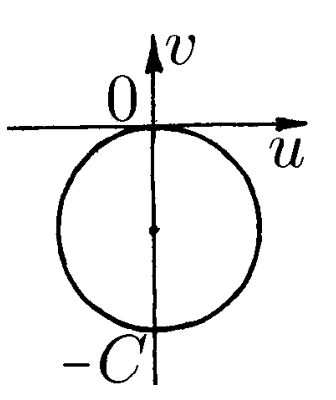
\includegraphics[width=.18\linewidth]{figures/figure-14.png}
\caption{}\label{q5:fig-14}
\end{figure}
или
\[
m\frac{\partial f}{\partial t}+\grad f\cdot\grad\varphi=0.
\]
Воспользовавшись постоянством давления на свободной поверхности и определением потенциала \eqref{q5:eq-8-1}, можно написать уравнение свободной поверхности в виде
\[
f(x,y,t)\equiv\varphi(x,y,t)+Cy+\mathrm{const}=0,
\]
подстановка которого в предыдущее уравнение дает условие на границе в нестационарном случае
\[
m\frac{\partial\varphi}{\partial t}+\left(\frac{\partial\varphi}{\partial x}\right)^2+\left(\frac{\partial\varphi}{\partial y}\right)^2+C\frac{\partial\varphi}{\partial y}=0.
\]
Отсюда при стационарной фильтрации на плоскости годографа получаем окружность радиуса $C/2$, проходящую через начало координат (рис.~\ref{q5:fig-14}):
\[
u^2+v^2+Cv=0.
\]

% Источник: Leontiev-2017.pdf; печатная страница: 47; страница файла: 47
\topic{Поверхность высачивания}
Для поверхности высачивания написать условие на потенциал $w$, не содержащее координат $x$, $y$, не удается, а в плоскости годографа образ границы можно построить в случае \textit{прямолинейной} границы. Умножая закон Дарси
\[
\boldsymbol{u}=-C\grad\left(\frac{p}{\rho g}+y\right)
\]
на касательный вектор к границе $\boldsymbol{\tau}$, получим, учитывая постоянство давления вдоль границы,
\[
\boldsymbol{u}\cdot\boldsymbol{\tau}=-C\tau_y=\mathrm{const},
\]
т.е. на плоскости $(u;v)$ концы вектора скорости лежат на прямой, перпендикулярной границе, но не проходящей, вообще говоря, через начало координат.

Приведем теперь примеры решения простейших задач.

\topic{Непроницаемая плотина с плоским основанием на пористом слое бесконечной глубины}
Рассмотрим стационарную фильтрацию жидкости через слой пористого материала, на котором находится непроницаемая плотина с плоским основанием длиной $2l$. Выберем начало координат в середине основания плотины (см. рис.~\ref{q5:fig-15}) и будем считать, что уровни жидкости $h_1$ и $h_2$ соответственно в нижнем и верхнем бьефах постоянны, а пористый слой простирается вниз до бесконечности.

\begin{figure}[H]
\centering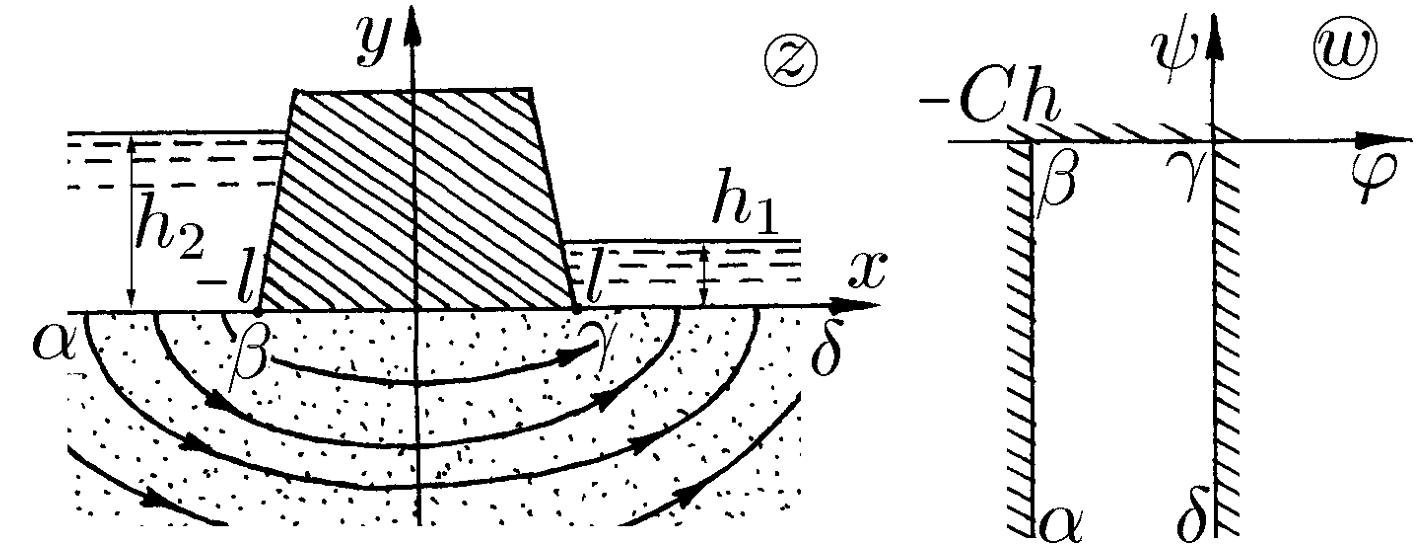
\includegraphics[width=.85\linewidth]{figures/figure-15.png}
\caption{}\label{q5:fig-15}
\end{figure}
В этой задаче область течения в плоскости комплексного потенциала $w$ полностью определена и является полубесконечной полосой: на непроницаемом основании плотины $\beta\gamma$ постоянна функция тока $\psi$, которую можно положить равной нулю, а на
% Источник: Leontiev-2017.pdf; печатная страница: 48; страница файла: 48
дне каждого из водоемов потенциалы скорости фильтрации $\varphi$ принимают постоянные значения. Если значение $\varphi$ на дне $\gamma\delta$ в нижнем бьефе принять равным нулю (добавление константы к $\varphi$ не меняет скорости фильтрации), то на дне $\alpha\beta$ в верхнем бьефе $\varphi=-C(h_2-h_1)=-Ch$, $h=h_2-h_1$.

Бесконечность функции тока при уходе на бесконечность (или, что то же самое, бесконечность расхода жидкости $Q$ в расчете на единицу длины плотины в направлении, перпендикулярном плоскости рисунка) следует уже из соображений размерности: предположение о конечности $Q$ приводит, после применения $\pi$-теоремы к зависимости $Q=f(Ch,l)$, к тому, что расход не зависит от размера плотины $l$: $Q=\mathrm{const}\cdot Ch$, но при стремлении ширины плотины к нулю ($l\to0$ при сохранении высоты плотины) решением задачи является вихрь $\varphi=\frac{Ch}{\pi}\theta$, где $\theta$ --- полярный угол, с бесконечным расходом, что и приводит к противоречию. Отметим, что если бы пористый пласт ограничивался снизу горизонтальной непроницаемой поверхностью, расположенной на конечной глубине, то в этом случае расход был бы конечным.

Если теперь нам удастся построить (какое-нибудь) конформное отображение нижней полуплоскости в физической плоскости $z$ на полуполосу в плоскости $w$, переводящее точки $\beta$, $\gamma$ и бесконечно удаленную точку $\alpha=\delta$ на плоскости $z$ в их соответствующие образы на плоскости $w$, то такое отображение и будет искомым, т.к. в комплексном анализе доказывается теорема о существовании и единственности конформного отображения области на область, переводящего любые три заданные граничные точки в любые три заданные граничные точки с сохранением порядка их обхода [9].

Несложно проверить, что требуемое отображение имеет вид
\begin{equation}
z=l\cos\left(\frac{\pi}{Ch}w(z)\right).
\tag{8.2}\label{q5:eq-8-2}
\end{equation}
Дифференцируя это соотношение и выражая производную $\frac{dw}{dz}$, получим комплексно-сопряженную скорость
\[
u-iv=\frac{dw}{dz}=-\frac{Ch}{\pi l}\frac{1}{\sin\bigl(\frac{\pi}{Ch}w(z)\bigr)}=-\frac{Ch}{\pi l}\frac{1}{\sqrt{1-z^2/l^2}},
\]
причем выбирается та ветвь квадратного корня, которая при $z=0$ дает положительную скорость $u=Ch/(\pi l)>0$. В частности,
% Источник: Leontiev-2017.pdf; печатная страница: 49; страница файла: 49
распределение скорости вдоль основания плотины имеет вид
\[
u(x)=\frac{Ch}{\pi}\frac{1}{\sqrt{l^2-x^2}},\qquad -l<x<l,
\]
на дне водоемов скорость фильтрации вертикальна:
\[
v(x)=\pm\frac{Ch}{\pi}\frac{1}{\sqrt{x^2-l^2}},\qquad |x|>l,
\]
(знаки «$+$» и «$-$» соответствуют нижнему и верхнему бьефам).

Обратим внимание, что в угловых точках основания направление скорости фильтрации меняется на $90^\circ$, а модуль скорости фильтрации стремится к бесконечности (как это бывает при обтекании углов в гидродинамике идеальной жидкости). В реальности, конечно, в силу разных причин (скругление углов дугами с конечными радиусами кривизны, отступление от закона Дарси, размытие грунта в области больших скоростей) скорости фильтрации в этих местах конечны.

Разделяя действительную и мнимую часть \eqref{q5:eq-8-2}\setcounter{footnote}{0}\footnote{Напомним, что $\cos(x+iy)=\cos x\cos(iy)-\sin x\sin(iy)=\cos x\operatorname{ch} y-i\sin x\operatorname{sh} y$.}:
\[
x=l\cos\widetilde\varphi\,\operatorname{ch}\widetilde\psi,\quad y=-l\sin\widetilde\varphi\,\operatorname{sh}\widetilde\psi,\quad
\widetilde\varphi=\frac{\pi\varphi}{Ch},\quad\widetilde\psi=\frac{\pi\psi}{Ch}
\]
и исключая $\varphi$, легко найти уравнение линий тока поля скорости фильтрации, которым соответствует постоянное значение $\psi$, --- эллипсов
\[
\left(\frac{x/l}{\operatorname{ch}\widetilde\psi}\right)^2+\left(\frac{x/l}{\operatorname{sh}\widetilde\psi}\right)^2=1.
\]
% В оригинале оба числителя содержат x/l; сохранено без исправления.
\begin{figure}[H]
\centering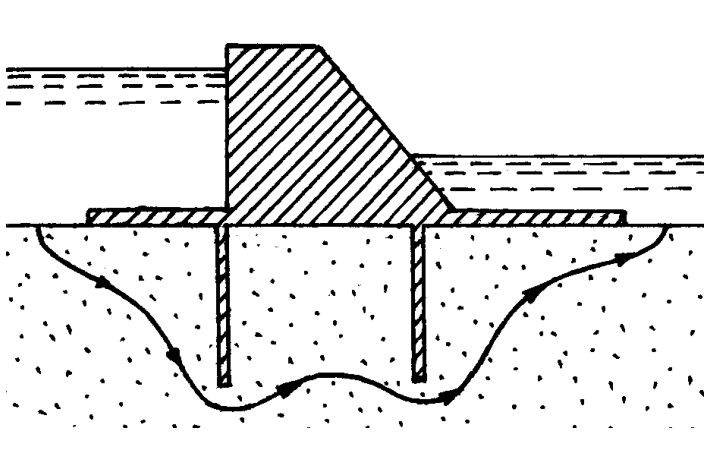
\includegraphics[width=.37\linewidth]{figures/figure-16.png}
\caption{}\label{q5:fig-16}
\end{figure}
Отметим, что реальные плотины являются сложными гидротехническими сооружениями, от основной подводной части которых отходят водонепроницаемые перегородки, идущие вдоль дна (так называемый \textit{пон\'ур}) или в глубину пласта (\textit{шпунтовые стенки}) и предназначенные для уменьшения скорости фильтрации под плотиной, ее закрепления в грунте и т.д. Качественно уменьшение скорости фильтрации можно объяснить тем,
% Источник: Leontiev-2017.pdf; печатная страница: 50; страница файла: 50
что жидкие частицы при своем движении вокруг выступов в подземной части плотины преодолевают больший путь, в то время как перепад напоров между начальной и конечной точками движения частиц остается неизменным (рис.~\ref{q5:fig-16}).

\topic{Приток к дренажной щели}
Приведем пример задачи с неизвестной свободной поверхностью. Рассмотрим безнапорный приток воды к полому горизонтальному каналу --- дрене\setcounter{footnote}{0}\footnote{Дрена (англ. drain --- «осушать») --- подземный искусственный водоток (труба, полость) для сбора и отвода почвенно-грунтовых вод. Дренажные системы, известные со времен Вавилона и Древнего Рима, применяются для осушения земель и борьбы с их засолением, для перехвата подземных вод и т.д. Пример простейшей дренажной системы, встречающейся в быту,--- отверстие на дне горшка для выращивания комнатных растений.}, который сделан в непроницаемом основании пористого пласта (часть поперечного сечения канала показана на рис.~\ref{q5:fig-17}).

\begin{figure}[H]
\centering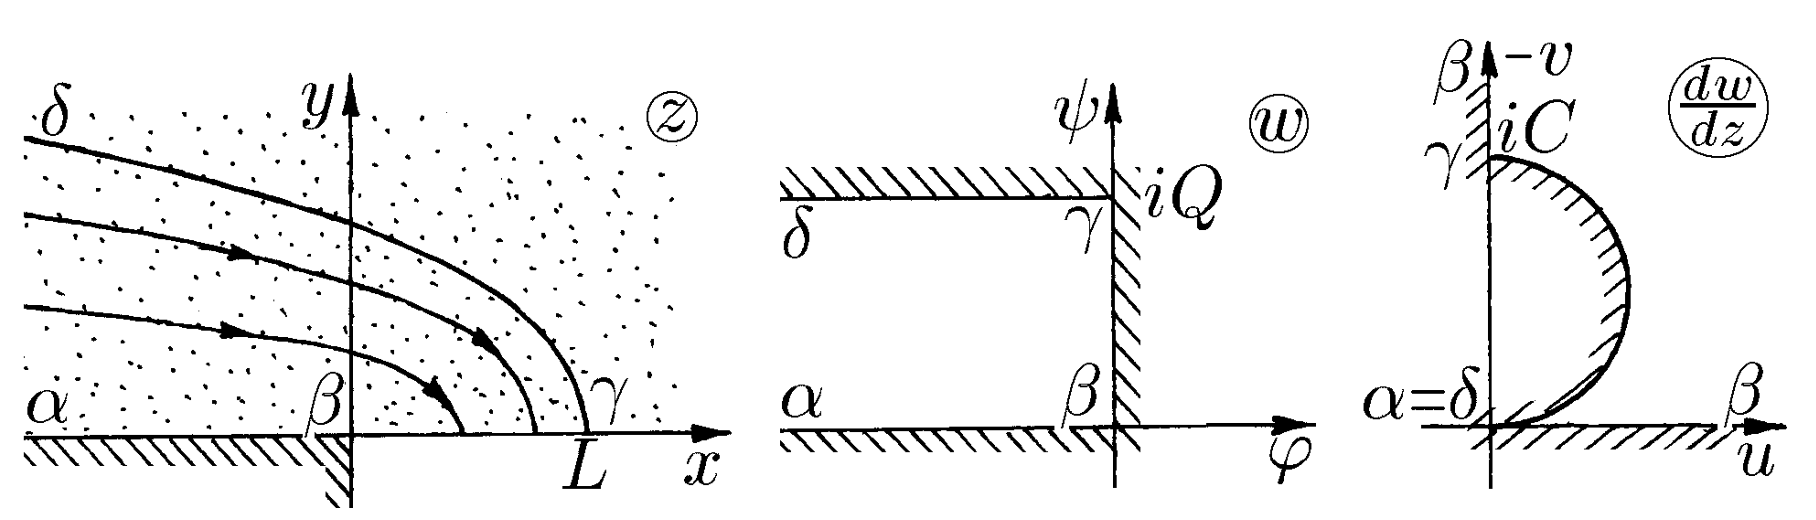
\includegraphics[width=.95\linewidth]{figures/figure-17.png}
\caption{}\label{q5:fig-17}
\end{figure}
Будем предполагать для простоты, что поток жидкости приходит из бесконечности, где высота поверхности депрессии стремится к бесконечности, а скорость фильтрации стремится к нулю, так что суммарный расход жидкости, фильтрующейся в пористой среде слева направо и собирающейся в полости дренажного канала, известен и равен конечной величине $Q$. Форма свободной поверхности на плоскости $z$ (и, в частности, длина $L$ промежутка высачивания $\beta\gamma$) заранее неизвестны, но образы области течения на плоскостях $w$ и $\frac{dw}{dz}$ легко находятся (рис.~\ref{q5:fig-17}; значения $\psi$ на непроницаемом основании $\alpha\beta$ и $\varphi$ на промежутке высачивания $\beta\gamma$ положены равными нулю, значение $\psi$ на свободной поверхности равно расходу $Q$). Отображение одной области на другую, построенное с соответствием точек $\alpha=\delta$, $\beta$ и $\gamma$, дает дифференциальное
% Источник: Leontiev-2017.pdf; печатная страница: 51; страница файла: 51
уравнение относительно $w(z)$:
\[
\frac{dw}{dz}=-\frac{CQ}{w},
\]
решение которого
\begin{equation}
w^2(z)=-2QCz+\mathrm{const}.
\tag{8.3}\label{q5:eq-8-3}
\end{equation}
Константа интегрирования равна нулю, т.к. точке $\beta$ на физической плоскости ($z=0$) соответствует точка $w=0$ на плоскости комплексного потенциала.

Теперь легко найти поле скоростей:
\[
u-iv=\frac{dw}{dz}=-\frac{CQ}{w}=-\sqrt{-\frac{CQ}{2z}},
\]
где нужно выбрать ветвь квадратного корня, дающую положительную скорость $u$ вдоль непроницаемого основания. Отсюда, в частности, для скорости фильтрации на непроницаемом основании получается зависимость
\[
u(x)=\sqrt{\frac{CQ}{2|x|}},\qquad x<0,
\]
а на промежутке высачивания
\[
v(x)=-\sqrt{\frac{CQ}{2x}},\qquad 0<x\leqslant L
\]
(в начале координат $|\boldsymbol{u}|$ обращается в бесконечность).

Уравнения линий тока и свободной поверхности получаются разделением действительной и мнимой частей в решении \eqref{q5:eq-8-3} и исключением потенциала скорости фильтрации $\varphi$, что дает уравнение параболы
\[
x=-\frac{CQ}{2\psi^2}y^2+\frac{\psi^2}{2CQ}
\]
(линиям тока соответствуют значения $0\leqslant\psi\leqslant Q$, поверхности депрессии --- $\psi=Q$, откуда при $y=0$ находится $L=Q/(2C)$).

% Источник: Leontiev-2017.pdf; печатная страница: 52; страница файла: 52
\topic{Течения в плоскости пласта}
Аналогичным образом методы теории аналитических функций применяются при рассмотрении плоскопараллельных горизонтальных течений в плоскости тонкого пласта. В этом случае координатная плоскость $Oxy$ располагается горизонтально, течение описывается уравнениями
\[
\triangle\varphi(x,y)=0,\quad\varphi=-CH(x,y),\quad C=\mathrm{const},\quad\boldsymbol{u}=\grad\varphi,
\]
где напор $H(x,y)=p(x,y,z)/(\rho g)+z$, в силу закона Дарси и предположения о плоскопараллельности течения, не меняется поперек пласта (при этом внутрипластовое давление вдоль любой вертикальной прямой $x=\mathrm{const}$, $y=\mathrm{const}$ распределено по гидростатическому закону).

Простейшие течения, встречающиеся на практике, --- поступательное течение в пласте со скоростью фильтрации $\boldsymbol{U}=(U_x;U_y)$ и течение вокруг работающей совершенной скважины, которое рассматривалось в конце § 7, описываются соответственно комплексными потенциалами $w(z)=\overline{U}z$ и $w(z)=Q/(2\pi)\ln z$, где $U=U_x+iU_y$, а черта над числом обозначает комплексное сопряжение. В силу линейности уравнений можно рассматривать линейные комбинации этих и других решений, что позволяет изучать, например, задачи о гидродинамическом взаимодействии группы скважин.

\topic{Скважина в поступательном потоке}
Рассмотрим в качестве примера работу скважины, откачивающей часть жидкости из фильтрационного потока с постоянной скоростью фильтрации $U=U_x$ на бесконечности. Картина течения в этом случае строится с помощью комплексного потенциала
\[
w(z)=Uz-\frac{Q}{2\pi}\ln z
\]
и имеет вид, показанный слева на рис.~\ref{q5:fig-18}. Скважина забирает жидкость, движущуюся на бесконечности внутри полосы шириной $Q/U$, которую называют \textit{областью питания скважины}. Остальная жидкость огибает скважину и уходит в бесконечность. Распределение напора на оси $x$ дается зависимостью
\[
H(x)=\frac{1}{C}\left(-Ux+\frac{Q}{2\pi}\ln|x|\right),
\]
% Источник: Leontiev-2017.pdf; печатная страница: 53; страница файла: 53
качественный вид которой показан справа на рис.~\ref{q5:fig-18}; локальный максимум на графике соответствует точке торможения потока.

Обратим внимание, что в этом решении при уходе в бесконечность в направлении оси $x$ давление в пласте рано или поздно станет равным нулю и, строго говоря, решение не будет справедливым во всей плоскости. Это связано с тем, что для поддержания потока в пористой среде нужно каким-либо образом создавать перепад давления, а для течения во всей плоскости, с формальной точки зрения, нужно было бы создать бесконечный перепад давления. Ситуация здесь совершенно аналогична движению вязкой жидкости в трубопров\'оде, где для поддержания течения на достаточно протяженном участке нужно поднимать давление с помощью насосов, расположенных на определенных расстояниях друг от друга.

\begin{figure}[H]
\centering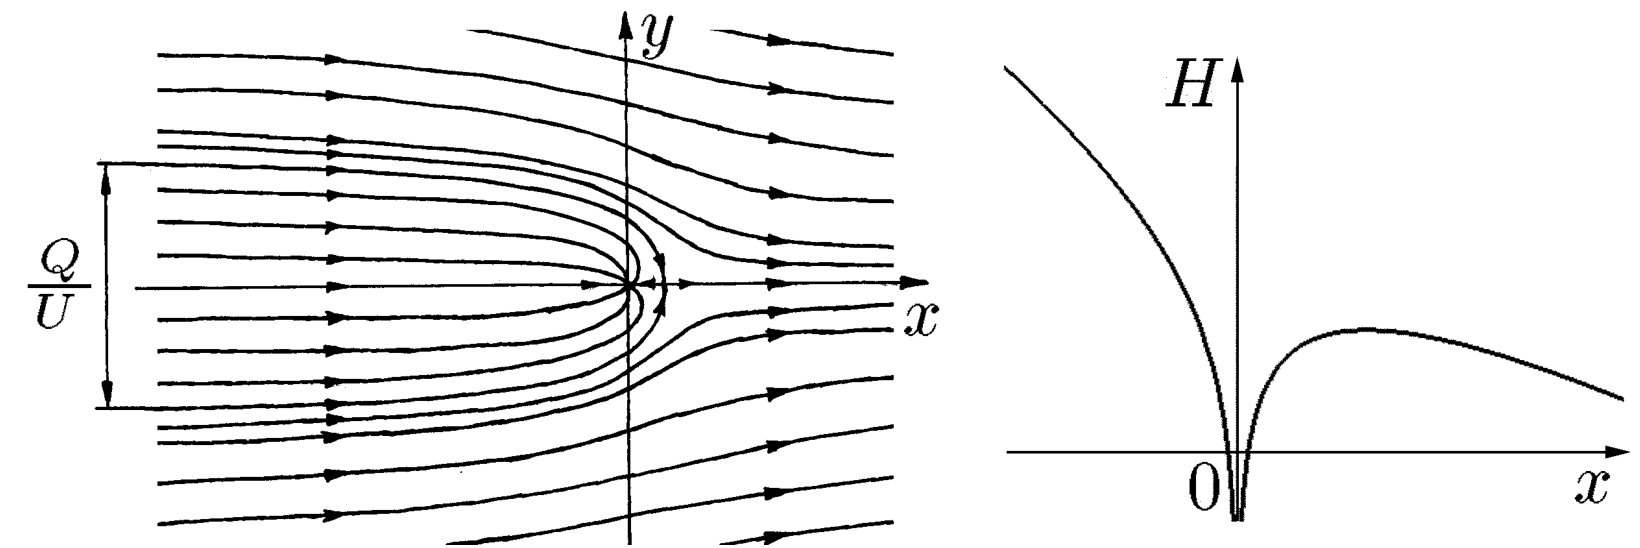
\includegraphics[width=.9\linewidth]{figures/figure-18.png}
\caption{}\label{q5:fig-18}
\end{figure}
\topic{О сходстве и различии фильтрационных течений и потенциальных течений идеальной жидкости}
Во избежание недоразумений подчеркнем, что несмотря на формальное совпадение кинематических уравнений для описания \textit{полей скорости} в теории фильтрации и в гидродинамике идеальной несжимаемой жидкости (в обоих случаях это уравнение Лапласа), распределение \textit{давления}, которое в отсутствие массовых сил является основной причиной движения, в этих моделях \textit{разное}.

Такое различие связано с тем, что эти модели отражают \textit{совершенно разные физические механизмы}: в \textit{фильтрационных} течениях (в области применимости закона Дарси) доминируют, как об этом уже говорилось, \textit{вязкие} силы, что связано с очень большой площадью поверхности пор, тогда как модель \textit{идеальной жидкости} учитывает явление другой природы --- \textit{инерцию} жидкости. Это различие проявляется уже в
% Источник: Leontiev-2017.pdf; печатная страница: 54; страница файла: 54
простейшем стационарном течении в горизонтальном цилиндрическом канале: в пористой среде давление падает вдоль канала, в то время как при течении идеальной жидкости градиенты давления вдоль канала отсутствуют.
% Конец § 8. Далее на странице 54 начинается § 9 «Гидравлическая теория безнапорной фильтрации».

\clearpage
\section*{Приложение. Труба-источник}
\noindent\textit{Источник: porous-lecture-notes.pdf, страницы файла 14--15. Автор, год и названия главы и параграфа в выбранном фрагменте не указаны. Видимые номера разворотов: 14 и 15. Это отдельный источник, не текст учебника Леонтьева.}
\par\medskip
% Источник: porous-lecture-notes.pdf; печатная страница: неизвестна; страница файла: 14; видимый рукописный номер разворота: 14
2. На $z$ форма области течения неизвестна.

Интенсивность источника $2Q$.

\begin{center}
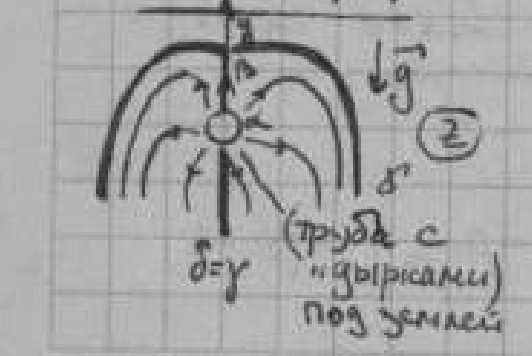
\includegraphics[width=.38\linewidth]{figures/notes-physical-domain.png}
\hspace{.04\linewidth}
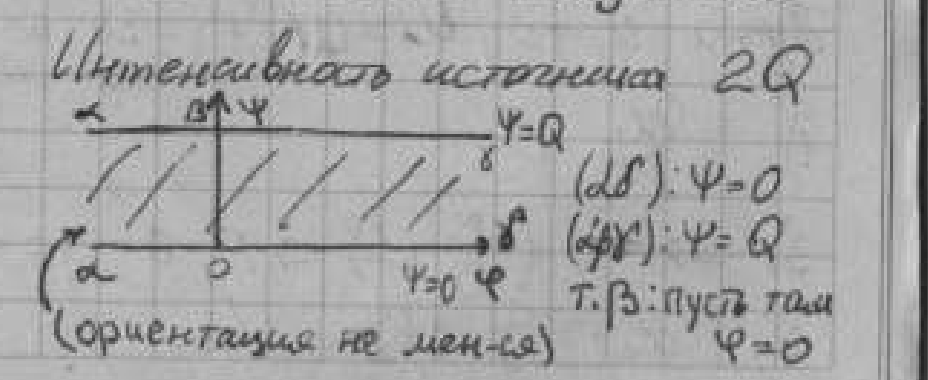
\includegraphics[width=.54\linewidth]{figures/notes-potential-domain.png}
\end{center}
Труба с «дырками» под землей.

\[
(\alpha\delta):\ \psi=0,\qquad(\beta\gamma):\ \psi=Q.
\]
Т. $\beta$: пусть там $\varphi=0$.

(ориентация не мен-ся)

% Источник: porous-lecture-notes.pdf; печатная страница: неизвестна; страница файла: 15; видимый рукописный номер разворота: 15
\begin{center}
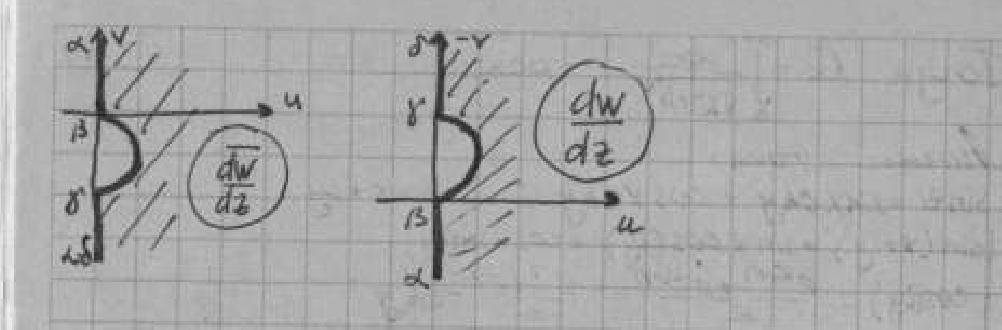
\includegraphics[width=.85\linewidth]{figures/notes-hodographs.png}
\end{center}
% На странице файла 15 включены только два рисунка-образа области течения, продолжающие постановку задачи на странице 14. Далее начинается «Гидравлическая теория ф-ции», не входящая в выбранный фрагмент.

\end{document}
